\documentclass[uplatex,dvipdfmx,ja=standard,twocolumn]{bxjsarticle}

\usepackage{graphicx}
\usepackage{times}
\usepackage[ms]{pxchfon}
\usepackage{titlesec}
\usepackage{amsmath}
\usepackage[shortlabels]{enumitem}
\usepackage{indentfirst}

\setpagelayout*{top=35truemm,bottom=27truemm,left=17.2truemm,right=17.2truemm}

\makeatletter
\def\@maketitle{%
\newpage\null
\vspace{-25pt}
\begin{center}%
  \let\footnote\thanks
  {\LARGE \@title \par}%
  \ifx\bxjs@subtitle\@undefined\else
    \vskip3\p@?
    {\normalsize \bxjs@subtitle\par}
  \fi
  \vskip 1.5em
  {\large
    \lineskip .5em
    \begin{tabular}[t]{c}%
      \@author
    \end{tabular}\par}%
  \vskip 1em
  {\large \@date}%
\end{center}%
\par\vskip 1.5em
\ifvoid\@abstractbox\else\centerline{\box\@abstractbox}\vskip1.5em\fi
}

\def\@biblabel#1{(#1)}

\def\@arabicz#1{\ifcase#1 0\or 1\or 2\or 3\or 4\or 5\or 6\or 7\or 8\or 9\else\@ctrerr\fi}
\def\arabicz#1{\expandafter\@arabicz\csname c@#1\endcsname}
\def\@arabicr#1{\ifcase#1\or ①\or ②\or ③\or ④\or ⑤\or ⑥ \or ⑦\or ⑧\or ⑨\else\@ctrerr\fi\relax}
\def\arabicr#1{\@arabicr{\@nameuse{c@#1}}}

\def\fnum@Jfigure{図}
\def\fnum@Efigure{Fig.}
\def\fnum@Jtable{表}
\def\fnum@Etable{Table}

\newcommand{\ieejcaption}[2]{%
\stepcounter{\@captype}
\par
\fontsize{8pt}{0pt}\selectfont
\csname fnum@J\@captype\endcsname \csname the\@captype\endcsname #1\par
\csname fnum@E\@captype\endcsname \csname the\@captype\endcsname. #2\par
}

\renewenvironment{thebibliography}[1]{%
  \@jsc@warnoldfontcmdexceptiontrue
  \global\let\presectionname\relax
  \global\let\postsectionname\relax
  \section*{\fontsize{8pt}{0pt}\selectfont \centerline{\refname}}\@mkboth{\refname}{\refname}%
  \vspace{-20pt}
  \hrule
  \vspace{8pt}
   \list{\@biblabel{\@arabic\c@enumiv}}%
    {\settowidth\labelwidth{\@biblabel{#1}}%
      \leftmargin\labelwidth
      \advance\leftmargin\labelsep
      \@openbib@code
      \usecounter{enumiv}%
      \let\p@enumiv\@empty
      \renewcommand\theenumiv{\@arabic\c@enumiv}}%
   \sloppy
   \clubpenalty4000
   \@clubpenalty\clubpenalty
   \widowpenalty4000%
   \sfcode`\.\@m}
  {\def\@noitemerr
    {\@latex@warning{Empty `thebibliography' environment}}%
    \endlist}
\makeatother

\renewcommand{\thesection}{\arabicz{section}.}
\renewcommand{\thesubsection}{<$\!$\arabic{section}・\arabic{subsection}$\!$>}
\renewcommand{\labelitemi}{・}
\renewcommand{\refname}{文 献}

\titleformat{\section}{\fontsize{11pt}{20pt}\bfseries}{\thesection}{0em}{}
\titlespacing*{\section}{0pt}{0pt}{0pt}
\titleformat{\subsection}[runin]{}{\thesubsection}{0em}{}[  ]

\setlength{\columnsep}{7mm}
\setlength{\labelsep}{3pt}
\setlength{\parindent}{0pt}
\setlist[itemize]{topsep=0pt,partopsep=0pt,leftmargin=9.8pt}
\setlist[enumerate]{topsep=0pt,partopsep=0pt,leftmargin=20pt,labelsep=0pt}
\AddEnumerateCounter{\arabicr}{\@arabicr}{①}
\SetEnumerateShortLabel{m}{\arabicr*}
\pagestyle{empty}

\title{\fontsize{19.5pt}{25pt}\selectfont 電気学会全国大会講演論文の書き方\vspace{8pt}}

\author{\fontsize{13pt}{14pt}\selectfont 研究 花子\textsuperscript{\!*},電気 太郎,学会 次郎 (○○○大学)\\
\fontsize{9pt}{14pt}\selectfont \\
\fontsize{9pt}{14pt}\selectfont Preparation of Papers for National Convention of I.E.E JAPAN\\
\fontsize{9pt}{14pt}\selectfont Hanako Kenkyu, Taro Denki, Jiro Gakkai (○○○University)}

\date{\vspace{-19pt}}

\begin{document}
\maketitle

\fontsize{9.8pt}{14pt}\selectfont

\section{まえがき}

 発表論文原稿は、A4原寸で印刷されます。
執筆の時は以下の説明をよく読んだ上で、お使いのワードプロセッサ等で可能な範囲で指示に従って原稿をお書きください。
なお、この説明書は、講演論文のレイアウトの見本になっていますので、参考にしてください。

\section{12年大会からの変更点}

 刷り上りの論文集の体裁は従来通りですが、以下の点が変更になっていますので注意してください。
\begin{itemize}
  \item 15年大会からPDF投稿を可能としました。
  \item 紙面投稿の場合専用の原稿用紙はありません。お手持ちのA4判白色の上質紙に印刷してください。
  \item 提出いただいた原稿は、CD-ROMを作成する際の原版としても使用します。CD-ROMはカラーが可能ですが、印刷論文集は白黒となります。ただし黄色などは印刷時に出力されないので、著者が白黒でプリントアウトして確認して下さい。
\end{itemize}

\section{レイアウトと文字サイズ}

\subsection{マージンとカラム幅}

原稿用紙のマージンおよびカラム幅(全ページ共通)は、表1のとおりです。
特に上下左右のマージンは厳守してください。

\vspace{-5pt}

\begin{table}[h]
  \centering
  \ieejcaption{マージン}{Margins}
  \fontsize{8pt}{12pt}\selectfont
  \begin{tabular}{lr}
    \hline
    上マージン       & 30mm\\
    下マージン       & 27mm\\
    左右マージン     & 18mm\\
    カラム間マージン &  7mm\\
    カラム幅         & 83.5mm\\
    \hline
  \end{tabular}
\end{table}

\vspace{-13pt}

\begin{table}[h]
  \fontsize{8pt}{10pt}\selectfont
  \centering
  \ieejcaption{文字サイズ}{Type sizes}
  \begin{tabular}{lll}
    \hline
                           & サイズ & 行送り\\
    論文タイトル           & 18pt   & 28pt\\
    著者名                 & 12pt   & 18pt\\
    英文タイトル著者所属名 &  9pt   & 14pt\\
    章タイトル             & 10pt   & 20pt\\
    本文                   &  9pt   & 14pt\\
    参考文献               &  8pt   & 12pt\\
    \hline
  \end{tabular}
\end{table}

\vspace{-10pt}

2カラム(2段組)とし、各コラムの幅、カラム間マージンは表1のとおりです。
本文の字詰は、1行あたり26文字程度とします。
分量は、図面、写真等を含めて1枚ないし2枚、シンポジウムは4枚以内です。

\subsection{配置}

表題等は、この見本に従って次の①~④の順序で記載し、本文を書き始めてください。
(2ページ目以降は、①~③不要)文字サイズと行送りは、表2を参考にしてください。

\begin{enumerate}[m]
  \item 表題:第1行中央に2カラム通しで書く(長ければ第2行も使う。第1行で済めば、第2行目は詰める)。\\表題1行目の左に、講演番号のスペースをあける。(テンプレートにおいては講演番号のスペースは設定してある)
  \item 著者名および勤務先:表題の下を1行あけて、次の行から中央に2カラム通しで書く。講演者名の右肩に「*」印を付ける。
  \item 英文表題、氏名(所属):著者名および勤務先の下を1行あけて、次の行から中央に2カラム通しで書く。
  \item 本文:英文による表題、氏名の下を1行あけて、次の行から書く。2ページは、上マージンに続いて第1行から本文を書く。
\end{enumerate}

\subsection{文献}

文献は本文末尾に通し番号を付けて一括記載し、本文中の該当個所に引用番号を付けてください。文献の記載方法は、著者名、雑誌名、ページ、発行年の順序にしてください。

\subsection{式および図}

式および図は、図1および以下の記載例を参考にしてください。図面等を貼り付ける場合は、しわにならないように注意してください。また、図および表の説明には、英文を併記してください。
\begin{equation}
  E = RI
\end{equation}
\begin{equation}
  V = Ri + L \frac{di}{dt}
\end{equation}

\vspace{-10pt}

\begin{figure}[h]
  \centering
  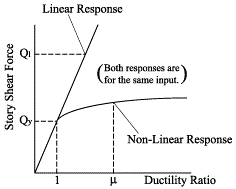
\includegraphics[height=23mm]{figure.png}
  \ieejcaption{図面の例}{An example of figures}
\end{figure}

\begin{thebibliography}{99}
\fontsize{8pt}{12pt}\selectfont

\bibitem{b1}
B Shahzadi: Electron, Eng., 63. 32~35 (1965)

\bibitem{b2}
天野一夫・有竹次男・角替四郎:昭50電気学会全大、No.508

\end{thebibliography}

\end{document}
